\documentclass[12pt]{article}

\usepackage[utf8]{inputenc}
\usepackage{latexsym,amsfonts,amssymb,amsthm,amsmath}
\usepackage{tikz}
\usepackage{stanli}
\usetikzlibrary{shapes,calc,through,3d,patterns}
\usetikzlibrary{arrows.meta,decorations.pathreplacing,angles,quotes}
\usepackage{multicol}
\usepackage{geometry}
\usepackage{mathtools}
\usepackage{siunitx}
\usepackage{booktabs}

\setlength{\parindent}{0in}
\setlength{\oddsidemargin}{-0.25in}
\setlength{\textwidth}{7in}
\setlength{\textheight}{9.3in}
\setlength{\topmargin}{-1in}
\setlength{\headheight}{18pt}

\newcommand\blfootnote[1]{%
    \begingroup
    \renewcommand\thefootnote{}\footnote{#1}%
    \addtocounter{footnote}{-1}%
    \endgroup
}

\definecolor{darkred}{rgb}{0.6,0,0}

\newcommand{\bolddelta}{\boldsymbol\delta}
\newcommand{\boldxi}{\boldsymbol\xi}

\begin{document}

\noindent ME473 - Dynamic finite element analysis of structures\hfill EPFL\\
Stefano Burzio \hfill 2025\\
\vspace{0.3cm}

\hspace*{\fill}\textbf{\Large Problem set 10}\hspace*{\fill}

\hrulefill

\subsection*{Problem 1}
We consider the dynamic response of a one-dimensional elastic bar of length \( \ell \), which is clamped at its left end and free at the right. The bar possesses a constant cross-sectional area \( A \), Young’s modulus \( E \), and mass density \( \rho \). It is assumed to be initially at rest, with zero displacement and velocity at time \( t = 0 \).

The bar is discretized using a single quadratic finite element with three equally spaced nodes. The configuration, including external dampers, is shown in figure below.
\begin{figure}[h!]
  \centering
  \begin{tikzpicture}[scale=1]
    \point{a}{0}{0};
    \support {3}{a}[270];
    % Draw the rectangle
    \filldraw[fill=gray!40, draw=black,thick] (0,-0.6) rectangle (10,0.6);
    %axis
    \draw[-latex, ultra thin] (0,0) -- (11,0) node[right]{$x$};
    % length
    \draw[ultra thin] (10,0) -- (10, 1.3) ;
    \draw[ultra thin] (0,-1.3) -- (0,1.3);
    \draw[latex-latex, ultra thin]  (0,1)  to node[sloped,midway,above] {$\ell$}(10,1) ;
    \draw[ultra thin]  (7,-0.3) -- (8,-1.2) node[right]{$E,A,\rho$};

    \fill (0,0) circle (3pt) node[below right] {$x_1$};
    \fill (10,0) circle (3pt) node[below right] {$x_3$};
    \draw[fill=white, draw=black] (5,0) circle (3pt) node[below right] {$x_2$};
  \end{tikzpicture}
  \label{fig:bar}
\end{figure}

Assuming a diagonal lumped mass matrix obtained by summing the columns of the consistent mass matrix, the structure stiffness and lumped mass matrices are given by:
\[
  \mathbf{K} = \frac{EA}{3\ell}
  \begin{bmatrix}
    7  & -8 & 1  \\
    -8 & 16 & -8 \\
    1  & -8 & 7
  \end{bmatrix}\qquad\text{and}\qquad
  \mathbf{M} = \frac{\rho A \ell}{6} \text{diag}(1, 4, 1).
\]
\begin{enumerate}
  \item Identify the unconstrained and constrained degrees of freedom of the structure.
  \item Assume an impulse force
        $$\mathbf r(t) = \begin{bmatrix}
            0 \\ 0\\ \delta(t)
          \end{bmatrix}$$
        is applied at the free end. Here $\delta(t)$ denotes the Dirac delta function. Using modal superposition, write the exact expression for the time response \(\mathbf q(t) \) of the system. \newline \textsc{Hint:} the mode shapes, normalized with respect to the diagonal mass matrix, are:
        \[
          \mathbf{p}_{1} = \frac{1}{\sqrt{\rho A \ell}}
          \begin{bmatrix}
            1.0066 \\
            1.3952
          \end{bmatrix}, \quad
          \mathbf{p}_{2} =\frac{1}{\sqrt{\rho A \ell}}
          \begin{bmatrix}
            -0.6976 \\
            2.0133
          \end{bmatrix}
        \]
  \item Consider the following data for the geometric and material properties of the bar:
        \vspace{-1cm}
        \begin{multicols}{2}
          \[
            \begin{aligned}
              \ell & = 1 \, \text{m} \quad        &  & \text{(length)}               \\
              A    & = 0.0001 \, \text{m}^2 \quad &  & \text{(cross-sectional area)} \\
            \end{aligned}
          \]

          \[
            \begin{aligned}
              E    & = 2.1 \times 10^{11} \, \text{Pa} \quad &  & \text{(Young's modulus)} \\
              \rho & = 7850 \, \text{kg/m}^3 \quad           &  & \text{(mass density)}    \\
            \end{aligned}
          \]
        \end{multicols}
        Using the average acceleration Newmark method ($\gamma = \frac{1}{2}, \, \beta = \frac{1}{4}$), compute the approximate solution to the modal equations at the initial time t = 0 and at the first time step $\Delta t = 0.1$ ms. This includes evaluating: the modal displacements $z_1(t)$, $z_2(t)$, the modal velocities $\dot{z}_1(t)$, $\dot{z}_2(t)$, and  the modal accelerations $\ddot{z}_1(t)$, $\ddot{z}_2(t)$,
        at $t = 0$ and $t = \Delta t$, based on the initial conditions and the discretized Newmark update scheme. Use the following approximation for the delta function
        $$\delta(t)=\begin{cases}
            1 & \text{if } t=0, \\
            0 & \text{if } t>0. \\
          \end{cases}$$
        Note that this is a numerical approximation of the Dirac delta function used solely to compute the initial response within the time-stepping scheme. It induces an instantaneous velocity jump at t = 0, and in general, such approximations should be avoided in favor of more physically realistic or regularized loading models.
\end{enumerate}
\end{document}